\documentclass[10pt]{beamer}

\usetheme[progressbar=frametitle]{metropolis}

\setbeamercolor{background canvas}{bg=white}
\usepackage{textpos}
\usepackage{booktabs}
\usepackage[scale=2]{ccicons}
\usepackage{amsmath} 
%\usepackage{animate}
\usepackage{multimedia}

\usepackage{pgfplots}
\usepgfplotslibrary{dateplot}
\usetikzlibrary{backgrounds}
\usepackage{xspace}
\newcommand{\themename}{\textbf{\textsc{metropolis}}\xspace}
\usepackage{caption}
\usepackage{booktabs}
\usepackage[scale=2]{ccicons}


\usepackage{tikz}
\usetikzlibrary{shapes,shadows,arrows,patterns, matrix, calc}
\usepackage[style=verbose,backend=biber]{biblatex}
\addbibresource{references.bib}

\tikzstyle{line} = [draw, -latex']
\tikzstyle{round} = [draw, circle, fill=black!30, minimum size=4em, node distance=4em, font=\fontsize{30}{10}\selectfont]
\tikzstyle{mlp_enc} = [rectangle, draw, fill=red!30, text width=2cm, minimum height=5em, text centered, node distance=10em, font=\fontsize{20}{10}\selectfont]
\tikzstyle{mlp_att} = [rectangle, draw, fill=green!30, text width=2cm, minimum height=5em, text centered, node distance=10em, font=\fontsize{20}{10}\selectfont]
\tikzstyle{mlp_dec} = [rectangle, draw, fill=blue!30, text width=2cm, minimum height=5em, text centered, node distance=10em, font=\fontsize{20}{10}\selectfont]
\tikzstyle{enc_h} = [rectangle, draw,  pattern=horizontal lines, pattern color=red!30, text width=1cm, minimum height=10em, minimum width=3em, text centered, node distance=10em, font=\fontsize{25}{10}\selectfont]
\tikzstyle{atts} = [rectangle, draw,  pattern=horizontal lines, pattern color=green!30, text width=1cm, minimum height=10em, minimum width=3em, text centered, node distance=10em, font=\fontsize{20}{10}\selectfont]
\tikzstyle{dec_z} = [rectangle, draw,  pattern=horizontal lines, pattern color=blue!30, text width=1cm, minimum height=10em, minimum width=3em, text centered, node distance=10em, font=\fontsize{20}{10}\selectfont]
\tikzstyle{cnn} = [rectangle, draw,  pattern=crosshatch, pattern color=red!50!blue!30, text width=2cm, minimum height=5em, text centered, node distance=10em, font=\fontsize{20}{10}\selectfont]
\tikzstyle{box} = [rectangle, draw,  fill=blue!20, text width=3cm, minimum height=5em, minimum width=3em, text centered, node distance=10em, font=\fontsize{20}{10}\selectfont]

\pgfdeclarelayer{background}
\pgfdeclarelayer{foreground}
\pgfsetlayers{background,main,foreground}

\usepackage{pgfplots}
\usepgfplotslibrary{dateplot}

\usepackage{xspace}


\title{Attention-based end-to-end models for ASR}
\subtitle{CTC, Attention and beyond}
\date{\today}
\author{Shreekantha A Nadig [MS2016010]}
\institute{Under the guidance of \\
	Prof. V.Ramasubramanian \\
	Prof. Sachit Rao}
 \titlegraphic{\hfill\includegraphics[height=1.5cm]{iiitb_logo.png}}

\begin{document}
	
\maketitle


\begin{frame}{Table of contents}
\setbeamertemplate{section in toc}[sections numbered]
\tableofcontents[hideallsubsections]
\end{frame}

\section{ASR}
\begin{frame}[fragile]{The Noisy Channel Model}
\begin{itemize}
	\item Search through space of all possible sentences.
	\item Pick the one that is most probable given the waveform.
\end{itemize}
\begin{figure}
	\includegraphics[width=\linewidth]{./images/page-04.png}
\end{figure}
\footcite{4767370}
\end{frame}


\begin{frame}[fragile]{The Noisy Channel Model}
\begin{itemize}
	\item What is the most likely sentence out of all sentences in the language L given some acoustic input O?
	\item Treat acoustic input O as sequence of individual observations $O = o_1, o_2, o_3, ... , o_T$
	\item Define a sentence as a sequence of words: $W = w_1, w_2, w_3, ... , w_U$
\end{itemize}
\end{frame}

\begin{frame}[fragile]{Raw audio}
\begin{itemize}
	\item Simple 1D signal:
	\begin{figure}
		\includegraphics[width=\linewidth]{./images/page-15.png}
	\end{figure}
	\item Typical sample rates for speech: 8KHz, 16KHz.
	\item Each sample typically 8-bit or 16-bit
	\item 1D vector: 
	$$\textbf{X} = [x_1, x_2, x_3, ... ]$$
\end{itemize}
\end{frame}


\begin{frame}[fragile]{Spectrogram}
\begin{itemize}
\item Take a small window (e.g., 20ms) of waveform

\item Compute FFT and take magnitude. (i.e., power)
\item Describes frequency content in local window.

\begin{figure}
	\includegraphics[width=\linewidth]{./images/page-17.png}
\end{figure}
\end{itemize}
\end{frame}


\begin{frame}[fragile]{Spectrogram}
\begin{itemize}
\item Concatenate frames from adjacent windows to form "spectrogram"
\begin{figure}
\includegraphics[width=\linewidth]{./images/page-18.png}
\end{figure}
\end{itemize}
\end{frame}

\begin{frame}[fragile]{The Noisy Channel Model - ASR equation}
\begin{itemize}
	\item Probabilistic implication: Pick the highest prob S:
	
	$$\hat{W} = \operatorname*{argmax}_{W \in L} P(W | O)$$
	\item We can use Bayes rule to rewrite this:
	$$\hat{W} = \operatorname*{argmax}_{W \in L} \frac{P(O | W)P(W)}{P(O)}$$
	
	\item Since denominator is the same for each candidate sentence W, we can ignore it for the argmax:
	$$\hat{W} = \operatorname*{argmax}_{W \in L} P(O | W)P(W)$$
	
\end{itemize}
\end{frame}



\section{Before end-to-end}

\begin{frame}[fragile]{Speech Recognition Architecture}
\begin{figure}
	\includegraphics[height=0.8\textheight]{./images/page-07.png}
\end{figure}
\end{frame}

\begin{frame}[fragile]{Acoustic Modeling with GMMs}
\begin{figure}
	\includegraphics[height=0.8\textheight]{./images/page-06.png}
\end{figure}
\end{frame}


\begin{frame}[fragile]{DNN Hybrid Acoustic Models}
\begin{figure}
\includegraphics[height=0.8\textheight]{./images/page-071.png}
\end{figure}
\end{frame}

\begin{frame}[fragile]{Recurrent DNN Hybrid Acoustic Models}
\begin{figure}
\includegraphics[height=0.8\textheight]{./images/page-09.png}
\end{figure}
\end{frame}


\begin{frame}[fragile]{HMM-Free Recognition}
\begin{figure}
	\includegraphics[height=0.8\textheight]{./images/page-11.png}
\end{figure}
\end{frame}


\begin{frame}[fragile]{Deep Recurrent Network}
\begin{figure}
\includegraphics[height=0.8\textheight]{./images/page-10.png}
\end{figure}
\end{frame}

\begin{frame}[fragile]{HMM-Free Recognition}
\begin{figure}
\includegraphics[height=0.8\textheight]{./images/page-12.png}
\end{figure}
\end{frame}

\begin{frame}[fragile]{Challenges in traditional ASR and Motivation for end-to-end}
\begin{itemize}
	\item Step-wise refinement (GMM-HMM -> DNN-HMM)
	\item Linguistic information (pronunciation dictionary)
	\item Conditional independence assumptions (Markov assumptions)
	\item Complex decoding (HCLG graph)
	\item Incoherence in optimization
	\item Traditional pipeline is highly tweakable, but also hard to get working well
	\item Historically, each part of system has own set of challenges (eg. choosing feature representation)
	\item Popular loss functions (MSE, XE) assume a one-to-one correspondence between the network’s output and target labels
	\item But what if there is no one-to-one correspondence? (Speech Recognition, Machine Translation, handwriting recognition)
	\item Need a way to find alignment between network outputs and target labels (CTC/Attention/seq2seq)
	\item Traditionally, try to bootstrap alignment - difficult!
\end{itemize}
\end{frame}

\section{End-to-end}
\begin{frame}[fragile]{BLSTM Encoder}
\begin{center}
	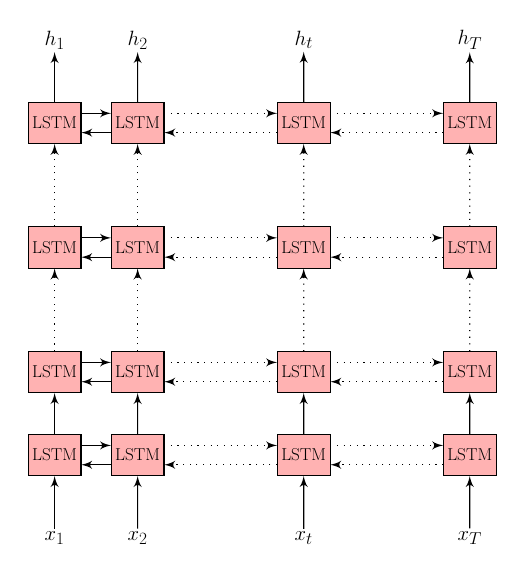
\begin{tikzpicture}[scale=0.3, every node/.style={transform shape}]
	\onslide<1->\node[mlp_enc](LSTM_1_1){LSTM};
	\node[mlp_enc, right of=LSTM_1_1](LSTM_1_2) {LSTM};
	\path [line] (LSTM_1_1.20) to (LSTM_1_1.20-|LSTM_1_2.west);
	\path [line] (LSTM_1_2.200) to (LSTM_1_2.-20-|LSTM_1_1.east);     
	
	\node[mlp_enc, right of=LSTM_1_2, node distance = 20em](LSTM_1_i) {LSTM};
	\path [line, dotted] (LSTM_1_2.20) to (LSTM_1_2.20-|LSTM_1_i.west);
	\path [line, dotted] (LSTM_1_i.200) to (LSTM_1_i.200-|LSTM_1_2.east);
	
	\node[mlp_enc, right of=LSTM_1_i, node distance = 20em](LSTM_1_Tx) {LSTM};
	\path [line, dotted] (LSTM_1_i.20) to (LSTM_1_i.20-|LSTM_1_Tx.west);
	\path [line, dotted] (LSTM_1_Tx.200) to (LSTM_1_Tx.200-|LSTM_1_i.east);
	
	\node [below of=LSTM_1_1, node distance = 10em, font=\fontsize{30}{10}\selectfont] (x1) {$x_{1}$};
	\node [below of=LSTM_1_2, node distance = 10em, font=\fontsize{30}{10}\selectfont] (x2) {$x_{2}$};
	\node [below of=LSTM_1_i, node distance = 10em, font=\fontsize{30}{10}\selectfont] (xi) {$x_{t}$};
	\node [below of=LSTM_1_Tx, node distance = 10em, font=\fontsize{30}{10}\selectfont] (xTx) {$x_{T}$};
	
	\path [line] (x1) to (LSTM_1_1);
	\path [line] (x2) to (LSTM_1_2);
	\path [line] (xi) to (LSTM_1_i);
	\path [line] (xTx) to (LSTM_1_Tx);
	
	\onslide<2->\node[mlp_enc, above of = LSTM_1_1](LSTM_2_1){LSTM};
	\node[mlp_enc, right of=LSTM_2_1](LSTM_2_2) {LSTM};
	\path [line] (LSTM_2_1.20) to (LSTM_2_1.20-|LSTM_2_2.west);
	\path [line] (LSTM_2_2.200) to (LSTM_2_2.-20-|LSTM_2_1.east);     
	
	\node[mlp_enc, right of=LSTM_2_2, node distance = 20em](LSTM_2_i) {LSTM};
	\path [line, dotted] (LSTM_2_2.20) to (LSTM_2_2.20-|LSTM_2_i.west);
	\path [line, dotted] (LSTM_2_i.200) to (LSTM_2_i.200-|LSTM_2_2.east);
	
	\node[mlp_enc, right of=LSTM_2_i, node distance = 20em](LSTM_2_Tx) {LSTM};
	\path [line, dotted] (LSTM_2_i.20) to (LSTM_2_i.20-|LSTM_2_Tx.west);
	\path [line, dotted] (LSTM_2_Tx.200) to (LSTM_2_Tx.200-|LSTM_2_i.east);
	
	\path [line] (LSTM_1_1) to (LSTM_2_1);
	\path [line] (LSTM_1_2) to (LSTM_2_2);
	\path [line] (LSTM_1_i) to (LSTM_2_i);
	\path [line] (LSTM_1_Tx) to (LSTM_2_Tx);
	
	\node[mlp_enc, above of = LSTM_2_1, node distance = 15em](LSTM_i_1){LSTM};
	\node[mlp_enc, right of=LSTM_i_1](LSTM_i_2) {LSTM};
	\path [line] (LSTM_i_1.20) to (LSTM_i_1.20-|LSTM_i_2.west);
	\path [line] (LSTM_i_2.200) to (LSTM_i_2.-20-|LSTM_i_1.east);     
	
	\node[mlp_enc, right of=LSTM_i_2, node distance = 20em](LSTM_i_i) {LSTM};
	\path [line, dotted] (LSTM_i_2.20) to (LSTM_i_2.20-|LSTM_i_i.west);
	\path [line, dotted] (LSTM_i_i.200) to (LSTM_i_i.200-|LSTM_i_2.east);
	
	\node[mlp_enc, right of=LSTM_i_i, node distance = 20em](LSTM_i_Tx) {LSTM};
	\path [line, dotted] (LSTM_i_i.20) to (LSTM_i_i.20-|LSTM_i_Tx.west);
	\path [line, dotted] (LSTM_i_Tx.200) to (LSTM_i_Tx.200-|LSTM_i_i.east);
	
	\path [line, dotted] (LSTM_2_1) to (LSTM_i_1);
	\path [line, dotted] (LSTM_2_2) to (LSTM_i_2);
	\path [line, dotted] (LSTM_2_i) to (LSTM_i_i);
	\path [line, dotted] (LSTM_2_Tx) to (LSTM_i_Tx);
	
	
	\onslide<4->\node[mlp_enc, above of = LSTM_i_1, node distance = 15em](LSTM_N_1){LSTM};
	\node[mlp_enc, right of=LSTM_N_1](LSTM_N_2) {LSTM};
	\path [line] (LSTM_N_1.20) to (LSTM_N_1.20-|LSTM_N_2.west);
	\path [line] (LSTM_N_2.200) to (LSTM_N_2.-20-|LSTM_N_1.east);     
	
	\node[mlp_enc, right of=LSTM_N_2, node distance = 20em](LSTM_N_i) {LSTM};
	\path [line, dotted] (LSTM_N_2.20) to (LSTM_N_2.20-|LSTM_N_i.west);
	\path [line, dotted] (LSTM_N_i.200) to (LSTM_N_i.200-|LSTM_N_2.east);
	
	\node[mlp_enc, right of=LSTM_N_i, node distance = 20em](LSTM_N_Tx) {LSTM};
	\path [line, dotted] (LSTM_N_i.20) to (LSTM_N_i.20-|LSTM_N_Tx.west);
	\path [line, dotted] (LSTM_N_Tx.200) to (LSTM_N_Tx.200-|LSTM_N_i.east);
	
	\path [line, dotted] (LSTM_i_1) to (LSTM_N_1);
	\path [line, dotted] (LSTM_i_2) to (LSTM_N_2);
	\path [line, dotted] (LSTM_i_i) to (LSTM_N_i);
	\path [line, dotted] (LSTM_i_Tx) to (LSTM_N_Tx);
	
	\onslide<5->\node [above of = LSTM_N_1, node distance = 10em, font=\fontsize{30}{10}\selectfont] (h1) {$h_{1}$};
	\node [above of = LSTM_N_2, node distance = 10em, font=\fontsize{30}{10}\selectfont] (h2) {$h_{2}$};
	\node [above of = LSTM_N_i, node distance = 10em, font=\fontsize{30}{10}\selectfont] (hi) {$h_{t}$};
	\node [above of = LSTM_N_Tx, node distance = 10em, font=\fontsize{30}{10}\selectfont] (hTx) {$h_{T}$};
	
	\path [line] (LSTM_N_1) to (h1);
	\path [line] (LSTM_N_2) to (h2);
	\path [line] (LSTM_N_i) to (hi);
	\path [line] (LSTM_N_Tx) to (hTx);
	\end{tikzpicture}
\end{center}
\end{frame}


\begin{frame}[fragile]{CTC - Connectionist Temporal Classification}
\begin{itemize}
	\item Maximum likelihood training of transcript
	\item Intuition: Alignments are unknown, so integrate over all possible time-character alignments
	$$L_{ctc}(X,W) = \sum_{C: k(C)=W}^{}p(C|X)$$
	$$= \sum_{C: k(C)=W}^{}\prod_{t=1}^{T}p(c_t|X)$$

	\item Example: W = "hi", T=3\\
	possible C such that k(C)=W:\\
	hhi,hii,\_hi,h\_i,hi\_
\end{itemize}
\end{frame}


%\begin{frame}[fragile]{CTC - Connectionist Temporal Classification}
%\begin{itemize}
%	\item Labels at each time index are conditionally independent (like HMMs)
%	$$Pr(a|x) = \prod_{t=1}^{T}Pr(a_t,t|x)$$
%	\item Sum over all time-level labelings consistent with the output label
%	$$Pr(y|x)=\sum_{a \in \beta^{-1}(y)}^{}Pr(a|x)$$
%	\item Final objective maximizes the probability of the true labels:
%	$$CTC(x) = -\log Pr(y^{*}|x)$$
%\end{itemize}
%\end{frame}

\begin{frame}[fragile]{CTC - Connectionist Temporal Classification}
\begin{itemize}
	\item RNN output neurons $c$ encode distribution over symbols.\\
	Note length(c) == length(x)
	\item For grapheme based model: $c \in \{A,B,C,D,...,Z,blank,space\}$
	\item Define a mapping $\beta(c) = y$
	\item Maximize likelihood of $y^{*}$ under this model
\end{itemize}
\begin{figure}
	\includegraphics[height=0.4\textheight]{./images/page-22.png}
\end{figure}


\begin{center}
	$$P(c=HHH\_E\_LL\_LO\_\_|x) = P(c_1=H|x)P(c_2=H|x) ... P(c_{15}=blank|x)$$
\end{center}

\end{frame}


\begin{frame}[fragile]{CTC - Connectionist Temporal Classification}
\begin{itemize}
	\item Define a mapping $\beta(c) -> y$
	\item Given a specific character sequence $c$, squeeze out duplicates + blanks to yield a transcription
	$$y = \beta(c) = \beta(HHH\_E\_LL\_LO\_\_) = "HELLO"$$
	\item Mapping implies a distribution over possible transcripts y:
	\begin{figure}
		\includegraphics[height=0.4\textheight]{./images/page-25.png}
	\end{figure}
\end{itemize}
\end{frame}


\begin{frame}[fragile]{CTC - Connectionist Temporal Classification}
\begin{itemize}
	\item Update network parameters $\theta$ to maximize the likelihood of correct label $y^{*}$
\end{itemize}
$$\theta^{*} =  \operatorname*{argmax}_{\theta} \sum_{i}^{} \log P(y^{*(i)}|x^{i}) = \operatorname*{argmax}_{\theta} \sum_{i}^{} \log \sum_{c:\beta(c)=y^{*}(i)}^{}P(c|x^{i})$$ \\
\begin{itemize}
	\item Graves et al., 2006 provides an efficient dynamic programming algorithm to compute the inner summation and it's gradients.
	\item Off-the-shelf packages to compute CTC loss from $c$, $y^{*}$ and gradients w.r.t. $c$
	\begin{itemize}
		\item Baidu's warp-ctc: "https://github.com/baidu-research/warp-ctc"
		\item PyTorch: "https://pytorch.org/docs/stable/nn.html\#ctcloss"
		\item TensorFlow: "https://www.tensorflow.org/api\_docs/python/tf/nn/ctc\_loss"
	\end{itemize}
	\item Getting RNN-CTC to train well is tricky
	\begin{itemize}
		\item Sortagrad - order utterances by length during first epoch
		\item Batch normalization
	\end{itemize}
\end{itemize}

%\begin{figure}
%	\includegraphics[height=0.3\textheight]{./images/page-27.png}
%\end{figure}

\end{frame}


%\begin{frame}[fragile]{CTC - Connectionist Temporal Classification}
%\animategraphics[autoplay,controls,loop,height=0.6\textheight, width=0.8\linewidth]{10}{./images/ctc/ctc-}{0}{178} 
%\end{frame}


\begin{frame}[fragile]{Basic Encoder-Decoder}
	\begin{center}
		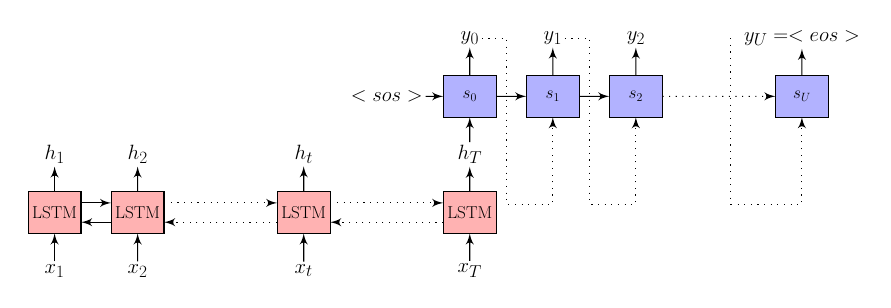
\begin{tikzpicture}[scale=0.3, every node/.style={transform shape}]
		\node[mlp_enc](LSTM_1_1){LSTM};
		\node[mlp_enc, right of=LSTM_1_1](LSTM_1_2) {LSTM};
		\path [line] (LSTM_1_1.20) to (LSTM_1_1.20-|LSTM_1_2.west);
		\path [line] (LSTM_1_2.200) to (LSTM_1_2.-20-|LSTM_1_1.east);     
		
		\node[mlp_enc, right of=LSTM_1_2, node distance = 20em](LSTM_1_i) {LSTM};
		\path [line, dotted] (LSTM_1_2.20) to (LSTM_1_2.20-|LSTM_1_i.west);
		\path [line, dotted] (LSTM_1_i.200) to (LSTM_1_i.200-|LSTM_1_2.east);
		
		\node[mlp_enc, right of=LSTM_1_i, node distance = 20em](LSTM_1_Tx) {LSTM};
		\path [line, dotted] (LSTM_1_i.20) to (LSTM_1_i.20-|LSTM_1_Tx.west);
		\path [line, dotted] (LSTM_1_Tx.200) to (LSTM_1_Tx.200-|LSTM_1_i.east);
		
		\node [below of=LSTM_1_1, node distance = 7em, font=\fontsize{30}{10}\selectfont] (x1) {$x_{1}$};
		\node [below of=LSTM_1_2, node distance = 7em, font=\fontsize{30}{10}\selectfont] (x2) {$x_{2}$};
		\node [below of=LSTM_1_i, node distance = 7em, font=\fontsize{30}{10}\selectfont] (xi) {$x_{t}$};
		\node [below of=LSTM_1_Tx, node distance = 7em, font=\fontsize{30}{10}\selectfont] (xTx) {$x_{T}$};
		
		\path [line] (x1) to (LSTM_1_1);
		\path [line] (x2) to (LSTM_1_2);
		\path [line] (xi) to (LSTM_1_i);
		\path [line] (xTx) to (LSTM_1_Tx);
		
		
		\node [above of = LSTM_1_1, node distance = 7em, font=\fontsize{30}{10}\selectfont] (h1) {$h_{1}$};
		\node [above of = LSTM_1_2, node distance = 7em, font=\fontsize{30}{10}\selectfont] (h2) {$h_{2}$};
		\node [above of = LSTM_1_i, node distance = 7em, font=\fontsize{30}{10}\selectfont] (hi) {$h_{t}$};
		\node [above of = LSTM_1_Tx, node distance = 7em, font=\fontsize{30}{10}\selectfont] (hTx) {$h_{T}$};
		
		\path [line] (LSTM_1_1) to (h1);
		\path [line] (LSTM_1_2) to (h2);
		\path [line] (LSTM_1_i) to (hi);
		\path [line] (LSTM_1_Tx) to (hTx);
		
		
		\node [mlp_dec, above of=hTx, node distance=7em] (dec0) {$s_{0}$};
		\node [left of=dec0, node distance = 10em, font=\fontsize{30}{10}\selectfont] (sos) {$<sos>$};
		\path [line] (sos.east) to (dec0.west);
		\path [line] (hTx) to (dec0);
		
		
		\node [above of=dec0, node distance = 7em, font=\fontsize{30}{10}\selectfont] (y0) {$y_{0}$};
		\path [line] (dec0) to (y0);
		
		
		\node [mlp_dec, right of=dec0] (dec1) {$s_{1}$};
		\path [line] (dec0.east) to (dec1.west);
		\node [above of=dec1, node distance = 7em, font=\fontsize{30}{10}\selectfont] (y1) {$y_{1}$};
		\path [line] (dec1) to (y1);
		\path [line, dotted] (y0.east) -- ++ (3em,0) -- ++ (0, -20em) -| (dec1);
		
		
		\node [mlp_dec, right of=dec1] (dec2) {$s_{2}$};
		\path [line] (dec1.east) to (dec2.west);
		\node [above of=dec2, node distance = 7em, font=\fontsize{30}{10}\selectfont] (y2) {$y_{2}$};
		\path [line] (dec2) to (y2);
		\path [line, dotted] (y1.east) -- ++ (3em,0) -- ++ (0, -20em) -| (dec2);
		
		
		\node [mlp_dec, right of=dec2, node distance = 20em] (decT) {$s_{U}$};
		\path [line, dotted] (y2.east) ++ (10em,0) -- ++ (0, -20em) -| (decT);
		\path [line, dotted] (dec2.east) to (decT.west);
		
		
		\node [above of=decT, node distance = 7em, font=\fontsize{30}{10}\selectfont] (yT) {$y_{U} = <eos>$};
		\path [line] (decT) to (yT);
		
		
		\end{tikzpicture}
	\end{center}
\end{frame}

\begin{frame}[fragile]{Encoder-Decoder}
	\begin{center}
		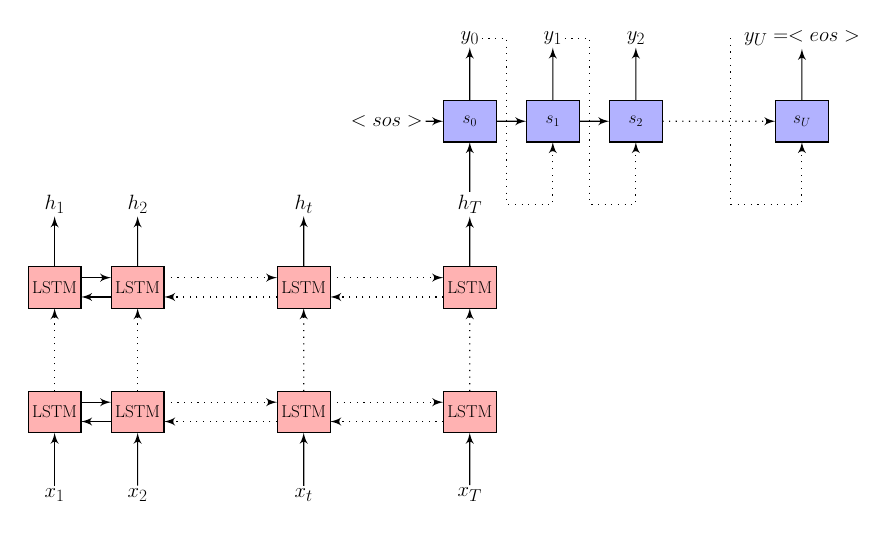
\begin{tikzpicture}[scale=0.3, every node/.style={transform shape}]
		\node[mlp_enc](LSTM_1_1){LSTM};
		\node[mlp_enc, right of=LSTM_1_1](LSTM_1_2) {LSTM};
		\path [line] (LSTM_1_1.20) to (LSTM_1_1.20-|LSTM_1_2.west);
		\path [line] (LSTM_1_2.200) to (LSTM_1_2.-20-|LSTM_1_1.east);     
		
		\node[mlp_enc, right of=LSTM_1_2, node distance = 20em](LSTM_1_i) {LSTM};
		\path [line, dotted] (LSTM_1_2.20) to (LSTM_1_2.20-|LSTM_1_i.west);
		\path [line, dotted] (LSTM_1_i.200) to (LSTM_1_i.200-|LSTM_1_2.east);
		
		\node[mlp_enc, right of=LSTM_1_i, node distance = 20em](LSTM_1_Tx) {LSTM};
		\path [line, dotted] (LSTM_1_i.20) to (LSTM_1_i.20-|LSTM_1_Tx.west);
		\path [line, dotted] (LSTM_1_Tx.200) to (LSTM_1_Tx.200-|LSTM_1_i.east);
		
		\node [below of=LSTM_1_1, node distance = 10em, font=\fontsize{30}{10}\selectfont] (x1) {$x_{1}$};
		\node [below of=LSTM_1_2, node distance = 10em, font=\fontsize{30}{10}\selectfont] (x2) {$x_{2}$};
		\node [below of=LSTM_1_i, node distance = 10em, font=\fontsize{30}{10}\selectfont] (xi) {$x_{t}$};
		\node [below of=LSTM_1_Tx, node distance = 10em, font=\fontsize{30}{10}\selectfont] (xTx) {$x_{T}$};
		
		\path [line] (x1) to (LSTM_1_1);
		\path [line] (x2) to (LSTM_1_2);
		\path [line] (xi) to (LSTM_1_i);
		\path [line] (xTx) to (LSTM_1_Tx);
		
		\pause{}
		\node[mlp_enc, above of = LSTM_1_1, node distance = 15em](LSTM_N_1){LSTM};
		\node[mlp_enc, right of=LSTM_N_1](LSTM_N_2) {LSTM};
		\path [line] (LSTM_N_1.20) to (LSTM_N_1.20-|LSTM_N_2.west);
		\path [line] (LSTM_N_2.200) to (LSTM_N_2.-20-|LSTM_N_1.east);     
		
		\node[mlp_enc, right of=LSTM_N_2, node distance = 20em](LSTM_N_i) {LSTM};
		\path [line, dotted] (LSTM_N_2.20) to (LSTM_N_2.20-|LSTM_N_i.west);
		\path [line, dotted] (LSTM_N_i.200) to (LSTM_N_i.200-|LSTM_N_2.east);
		
		\node[mlp_enc, right of=LSTM_N_i, node distance = 20em](LSTM_N_Tx) {LSTM};
		\path [line, dotted] (LSTM_N_i.20) to (LSTM_N_i.20-|LSTM_N_Tx.west);
		\path [line, dotted] (LSTM_N_Tx.200) to (LSTM_N_Tx.200-|LSTM_N_i.east);
		
		\path [line, dotted] (LSTM_1_1) to (LSTM_N_1);
		\path [line, dotted] (LSTM_1_2) to (LSTM_N_2);
		\path [line, dotted] (LSTM_1_i) to (LSTM_N_i);
		\path [line, dotted] (LSTM_1_Tx) to (LSTM_N_Tx);
		
		\pause{}
		\node [above of = LSTM_N_1, node distance = 10em, font=\fontsize{30}{10}\selectfont] (h1) {$h_{1}$};
		\node [above of = LSTM_N_2, node distance = 10em, font=\fontsize{30}{10}\selectfont] (h2) {$h_{2}$};
		\node [above of = LSTM_N_i, node distance = 10em, font=\fontsize{30}{10}\selectfont] (hi) {$h_{t}$};
		\node [above of = LSTM_N_Tx, node distance = 10em, font=\fontsize{30}{10}\selectfont] (hTx) {$h_{T}$};
		
		\path [line] (LSTM_N_1) to (h1);
		\path [line] (LSTM_N_2) to (h2);
		\path [line] (LSTM_N_i) to (hi);
		\path [line] (LSTM_N_Tx) to (hTx);
		
		\pause{}
		\node [mlp_dec, above of=hTx] (dec0) {$s_{0}$};
		\node [left of=dec0, node distance = 10em, font=\fontsize{30}{10}\selectfont] (sos) {$<sos>$};
		\path [line] (sos.east) to (dec0.west);
		\path [line] (hTx) to (dec0);
		
		\pause{}
		\node [above of=dec0, node distance = 10em, font=\fontsize{30}{10}\selectfont] (y0) {$y_{0}$};
		\path [line] (dec0) to (y0);
		
		\pause{}
		\node [mlp_dec, right of=dec0] (dec1) {$s_{1}$};
		\path [line] (dec0.east) to (dec1.west);
		\node [above of=dec1, node distance = 10em, font=\fontsize{30}{10}\selectfont] (y1) {$y_{1}$};
		\path [line] (dec1) to (y1);
		\path [line, dotted] (y0.east) -- ++ (3em,0) -- ++ (0, -20em) -| (dec1);
		
		\pause{}
		\node [mlp_dec, right of=dec1] (dec2) {$s_{2}$};
		\path [line] (dec1.east) to (dec2.west);
		\node [above of=dec2, node distance = 10em, font=\fontsize{30}{10}\selectfont] (y2) {$y_{2}$};
		\path [line] (dec2) to (y2);
		\path [line, dotted] (y1.east) -- ++ (3em,0) -- ++ (0, -20em) -| (dec2);
		
		\pause{}
		\node [mlp_dec, right of=dec2, node distance = 20em] (decT) {$s_{U}$};
		\path [line, dotted] (y2.east) ++ (10em,0) -- ++ (0, -20em) -| (decT);
		\path [line, dotted] (dec2.east) to (decT.west);
		
		\pause{}
		\node [above of=decT, node distance = 10em, font=\fontsize{30}{10}\selectfont] (yT) {$y_{U} = <eos>$};
		\path [line] (decT) to (yT);
		
		
		\end{tikzpicture}
	\end{center}
\end{frame}


\section{Attention}

\begin{frame}[fragile]{Attention}
\begin{figure}
	\includegraphics[width=\linewidth]{att_profile.png}
\end{figure}
\end{frame}


\begin{frame}[fragile]{Introduction to Attention}
	\begin{center}
		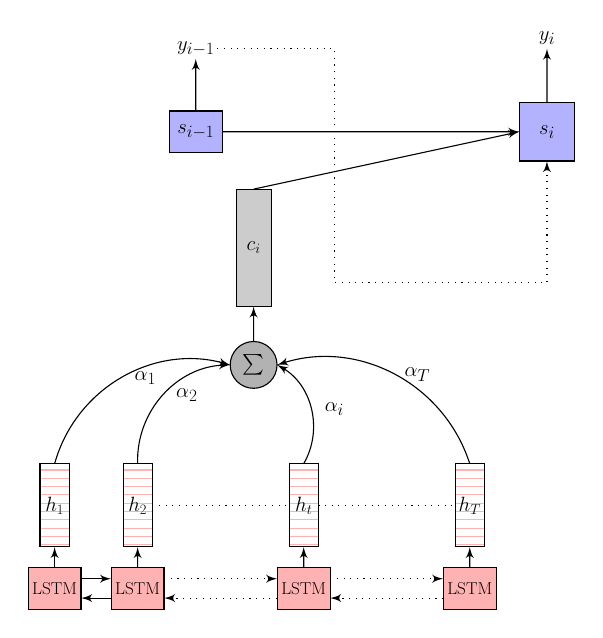
\begin{tikzpicture}[scale=0.3, every node/.style={transform shape}]
		\node[mlp_enc, node distance = 15em](LSTM_N_1){LSTM};
		\node[mlp_enc, right of=LSTM_N_1](LSTM_N_2) {LSTM};
		\path [line] (LSTM_N_1.20) to (LSTM_N_1.20-|LSTM_N_2.west);
		\path [line] (LSTM_N_2.200) to (LSTM_N_2.-20-|LSTM_N_1.east);     
		
		\node[mlp_enc, right of=LSTM_N_2, node distance = 20em](LSTM_N_i) {LSTM};
		\path [line, dotted] (LSTM_N_2.20) to (LSTM_N_2.20-|LSTM_N_i.west);
		\path [line, dotted] (LSTM_N_i.200) to (LSTM_N_i.200-|LSTM_N_2.east);
		
		\node[mlp_enc, right of=LSTM_N_i, node distance = 20em](LSTM_N_Tx) {LSTM};
		\path [line, dotted] (LSTM_N_i.20) to (LSTM_N_i.20-|LSTM_N_Tx.west);
		\path [line, dotted] (LSTM_N_Tx.200) to (LSTM_N_Tx.200-|LSTM_N_i.east);
		
		
		\node [enc_h, above of = LSTM_N_1] (h1) {$h_{1}$};
		\node [enc_h,above of = LSTM_N_2] (h2) {$h_{2}$};
		\node [enc_h,above of = LSTM_N_i] (hi) {$h_{t}$};
		\node [enc_h,above of = LSTM_N_Tx] (hTx) {$h_{T}$};
		
		\draw [dotted] (h2.east) to (hi.west);
		\draw [dotted] (hi.east) to (hTx.west);
		
		\path [line] (LSTM_N_1) to (h1);
		\path [line] (LSTM_N_2) to (h2);
		\path [line] (LSTM_N_i) to (hi);
		\path [line] (LSTM_N_Tx) to (hTx);
		
		\node [mlp_dec, above of = h1, node distance = 45em, xshift=17em, font=\fontsize{30}{10}\selectfont] (decoder_tm1) {$s_{i-1}$};
		\node [above of = decoder_tm1, node distance = 10em, font=\fontsize{30}{10}\selectfont] (ytm1) {$y_{i-1}$};
		\path [line] (decoder_tm1) to (ytm1);
		
		
		\pause{}
		\fontsize{15}{12}
		\node [round, above of = h1, node distance = 12em, xshift=17em] (sum1) {$\sum$};
		
		\pause{}
		\path [line] (h1.north) to [bend left=45] node [xshift=2em, font=\fontsize{30}{10}\selectfont] {$\alpha_{1}$} (sum1.west);
		\pause{}
		\path [line] (h2.north) to [bend left=45] node [xshift=2em, font=\fontsize{30}{10}\selectfont] {$\alpha_{2}$} (sum1.west);
		\pause{}
		\path [line] (hi.north) to [bend right=45] node [xshift=2em, font=\fontsize{30}{10}\selectfont] {$\alpha_{i}$} (sum1.east);
		\pause{}
		\path [line] (hTx.north) to [bend right=45] node [xshift=2em, font=\fontsize{30}{10}\selectfont] {$\alpha_{T}$} (sum1.east);
		
		\pause{}
		\node [enc_h, above of = sum1, fill=black!20] (ci) {$c_{i}$};
		
		\path [line] (sum1) to (ci.south);
		
		
		\pause{}
		\node [mlp_dec, right of = decoder_tm1, node distance = 30em, font=\fontsize{30}{10}\selectfont] (decoder_t) {$s_{i}$};
		\path [line] (decoder_tm1.east) to (decoder_t.west);
		\path [line] (ci.north) to (decoder_t.west);
		
		\path [line, dotted] (ytm1.east) -- ++ (10em,0) -- ++ (0, -20em) -| (decoder_t);
		\pause{}
		\node [above of = decoder_t, node distance = 8em, font=\fontsize{30}{10}\selectfont] (yt) {$y_{i}$};
		\path [line] (decoder_t) to (yt);
		\end{tikzpicture}
	\end{center}
\end{frame}

%\begin{frame}[fragile]{Introduction to Attention}
%\movie[loop,autostart,width=8cm,height=4.5cm]{test}{att_single_20_phns_progress.mp4}
%
%%\movie[loop,autostart]{\includegraphics[width=0.43\textwidth]{nadig_spml_att.pdf}}{}
%\end{frame}

%\begin{frame}[fragile]{Introduction to Attention 2}
%\href{run:att_dot.gif}{Click for video}
%Attention animated 2
%\end{frame}

\begin{frame}[fragile]{Attention}
\begin{block}{Attention}
	An attention function can be described as mapping a query and a set of key-value pairs to an output.
	Each time the model needs to generate an output symbol, it (soft-) searches for a set of positions in the input feature vector sequence where the most relevant information is concentrated.
\end{block}

\begin{itemize}
	\item The \textcolor{green}{query}, \textcolor{red!60}{keys}, \textcolor{red}{values}, and output are all vectors
	\item The output is computed as a weighted sum of the values, where the weight assigned to each value is computed by a compatibility function of the query with the corresponding key.
	\item Query : $dec_z \in \mathcal{R}^{d_q}$
	\item Key : $f(h) \in \mathcal{R}^{d_k}$
	\item Value : $g(h) \in \mathcal{R}^{d_v}$
	\item $Attention(Q,K,V) = Softmax(\dfrac{QK^T}{\sqrt{d_k}}) V$
\end{itemize}
Attention plots.
\end{frame}

\begin{frame}[fragile]{Attention}
\begin{itemize}
	\item $x = (x_{1}, x_{2}, .........., x_{T})$ is the input sequence
	\item $y = (y_{1}, y_{2}, .........., y_{U})$ is the target output sequence
	\item $h_{t} = f(x_{t}, h_{t-1})$ is the Encoder function
	\item $h = (h_{1}, h_{2}, .........., h_{T})$ is the output of the Encoder
	\item $C_{i} = \sum_{j=1}^{T} \alpha_{i,j} \cdot h_{j}$ is the Context vector
	\item $\alpha_{i,j} = Softmax(e_{i,j}) = \frac{e^{e_{i,j}}}{\sum_{k=1}^{T} e^{e_{i,k}}}$ are the Attention weights
	\item $e_{i,j} = a(s_{i-1}, h_j)$ is the importance parameter for every encoded input
	\item $\sum_{j=1}^{T} e_{i,j} \neq 1$ the importance parameter need not sum to 1
	\item $\sum_{j=1}^{T} \alpha_{i,j} = 1$ the attention weights sum to 1
	\item $p(y_{i} | \{y_1, y_2, .........., y_{i-1}\}, C_{i}) = g(y_{i-1}, s_i, C_{i})$ is the output symbol at the current time step
	\item $p(y) = \prod_{i=1}^{U} p(y_i | \{y_1, y_2, .........., y_{i-1}\}, C_{i})$ is the probability of the entire output sequence
\end{itemize}

\end{frame}

\begin{frame}[fragile]{Dot product Attention}
\begin{center}
	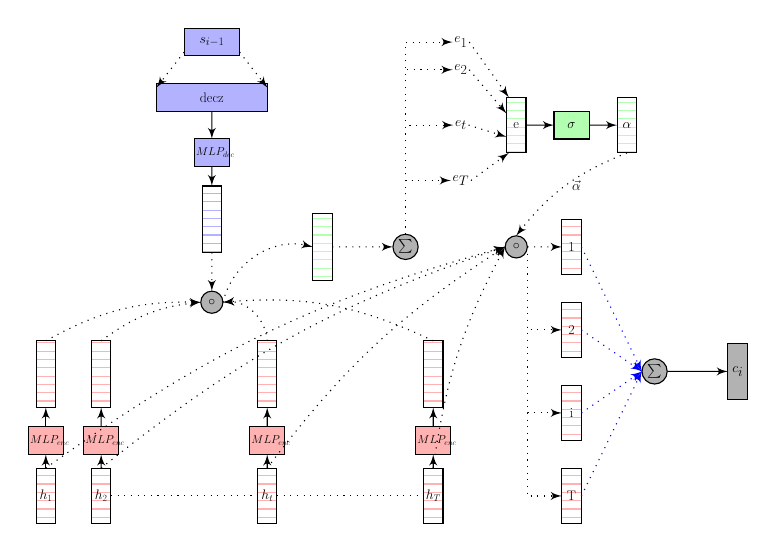
\begin{tikzpicture}[scale=0.2, every node/.style={transform shape}]
	\node [enc_h] (h1) {$h_{1}$};
	\node [enc_h,right of = h1] (h2) {$h_{2}$};
	\node [enc_h,right of = h2, node distance = 30em] (hi) {$h_{t}$};
	\node [enc_h,right of = hi, node distance = 30em] (hTx) {$h_{T}$};
	\draw [dotted] (h2.east) to (hi.west);
	\draw [dotted] (hi.east) to (hTx.west);
	
	
	\node [mlp_enc, above of = h1, node distance = 10em] (mlp1) {$MLP_{enc}$};
	\path [line] (h1.north) to (mlp1.south);
	\node [enc_h, above of = mlp1, minimum height = 12em, node distance = 12em] (he1) {};
	\path [line] (mlp1.north) to (he1.south);
	
	
	\node [mlp_enc, above of = h2, node distance = 10em] (mlp2) {$MLP_{enc}$};
	\path [line] (h2.north) to (mlp2.south);
	\node [enc_h, above of = mlp2, minimum height = 12em, node distance = 12em] (he2) {};
	\path [line] (mlp2.north) to (he2.south);
	
	
	\node [mlp_enc, above of = hi, node distance = 10em] (mlpi) {$MLP_{enc}$};
	\path [line] (hi.north) to (mlpi.south);
	\node [enc_h, above of = mlpi, minimum height = 12em, node distance = 12em] (hei) {};
	\path [line] (mlpi.north) to (hei.south);
	
	
	\node [mlp_enc, above of = hTx, node distance = 10em] (mlpTx) {$MLP_{enc}$};
	\path [line] (hTx.north) to (mlpTx.south);
	\node [enc_h, above of = mlpTx, minimum height = 12em, node distance = 12em] (heTx) {};
	\path [line] (mlpTx.north) to (heTx.south);
	
	\node [mlp_dec, above of = hei, node distance = 60em, minimum width = 10em, xshift = -10em, font=\fontsize{30}{10}\selectfont] (sim1) {$s_{i-1}$};
	\node [mlp_dec, below of=sim1, minimum width = 20em, font=\fontsize{40}{10}\selectfont] (dec_z) {decz};
	\path [line, dotted] (sim1.200) to (dec_z.170);
	\path [line, dotted] (sim1.-20) to (dec_z.10);
	\node [mlp_dec, below of=dec_z, node distance = 10em] (mlp_dec) {$MLP_{dec}$};
	\path [line] (dec_z) to (mlp_dec);
	\node [dec_z, below of = mlp_dec, minimum height = 12em, node distance = 12em] (decz_enc) {};
	\path [line] (mlp_dec) to (decz_enc);
	
	\uncover<2-7>{
		\node [round, below of = decz_enc, node distance = 15em] (prod) {$\circ$}; 
		\path [line, dotted] (decz_enc.south) to (prod.north);
		\uncover<2-4>{
			\path [line, dotted] (he1.north) to [bend left=15] (prod.west);
		}
		\node [atts, right of = prod, minimum height = 12em, node distance = 20em, yshift=10em] (h_z) {};
		\path [line, dotted] (prod.east) to [bend left=45] (h_z.west);
	}
	
	\uncover<3-7>{
		\node [round, right of = h_z, node distance = 15em] (sum) {$\sum$};
		\path [line, dotted] (h_z.east) to (sum.west);
	}
	
	\uncover<4->{
		\node [right of=sim1, node distance = 15em, xshift=30em, font=\fontsize{40}{10}\selectfont] (e1) {$e_{1}$};
		\uncover<4>{
			\path [line, dotted] (sum.north) |- (e1.west);
		}
	}
	
	\uncover<5->{
		\node [below of=e1, node distance = 5em, font=\fontsize{40}{10}\selectfont] (e2) {$e_{2}$};
		\uncover<5>{
			\path [line, dotted] (he2.north) to [bend left=15] (prod.west);
			\path [line, dotted] (sum.north) |- (e2.west);
		}
	}
	
	\uncover<6->{
		\node [below of=e2, node distance = 10em, font=\fontsize{40}{10}\selectfont] (ei) {$e_{t}$};
		\uncover<6>{
			\path [line, dotted] (hei.north) to [bend right=45] (prod.east);
			\path [line, dotted] (sum.north) |- (ei.west);
		}
	}
	
	\uncover<7->{
		\node [below of=ei, node distance = 10em, font=\fontsize{40}{10}\selectfont] (eTx) {$e_{T}$};
		\only<7>{
			\path [line, dotted] (heTx.north) to [bend right=15] (prod.east);
			\path [line, dotted] (sum.north) |- (eTx.west);
		}
	}
	
	\uncover<8->{
		\node [atts, right of=ei, font=\fontsize{40}{10}\selectfont] (e) {e};
		
		
		\path [line, dotted] (e1.east) to (e.105);
		\path [line, dotted] (e2.east) to (e.130);
		\path [line, dotted] (ei.east) to (e.-130);
		\path [line, dotted] (eTx.east) to (e.-105);
		
		
		\node [mlp_att, right of=e, font=\fontsize{40}{10}\selectfont] (sm) {$\sigma$};
		\path [line] (e.east) to (sm.west);
		
		
		\node [atts, right of=sm, font=\fontsize{40}{10}\selectfont] (alphas) {$\alpha$};
		\path [line] (sm.east) to (alphas.west);
	}
	
	\uncover<9>{
		\node [round, right of=sum, node distance=20em] (alpha_h) {$\circ$};
		\path [line, dotted, color=black] (h1.north) to [bend left=10] (alpha_h.west);
		\path [line, dotted, color=black] (alphas.south) to [bend right=15] node [xshift=2em] {\fontsize{40}{10}\selectfont $\vec{\alpha}$} (alpha_h.north);
		
		
		\node [enc_h, right of=alpha_h] (ahe1) {1};
		\path [line, dotted, color=black] (alpha_h.east) to (ahe1.west);
		
		\path [line, dotted, color=black] (h2.north) to [bend left=10] (alpha_h.west);
		\node [enc_h, below of=ahe1, node distance = 15em] (ahe2) {2};
		\path [line, dotted, color=black] (alpha_h.east) |- (ahe2.west);
		
		
		\path [line, dotted, color=black] (hi.north) to [bend left=10] (alpha_h.west);
		\node [enc_h, below of=ahe2, node distance = 15em] (ahei) {i};
		\path [line, dotted, color=black] (alpha_h.east) |- (ahei.west);
		
		\path [line, dotted, color=black] (hTx.north) to [bend left=10] (alpha_h.west);
		\node [enc_h, below of=ahei, node distance = 15em] (aheTx) {T};
		\path [line, dotted, color=black] (alpha_h.east) |- (aheTx.west);
		
		\pause{}
		\node [round, right of=ahe2, yshift=-7.5em, node distance = 15em] (sum_op) {$\sum$};
		\path [line, dotted, color=blue] (ahe1.east) to (sum_op.west);
		\path [line, dotted, color=blue] (ahe2.east) to (sum_op.west);
		\path [line, dotted, color=blue] (ahei.east) to (sum_op.west);
		\path [line, dotted, color=blue] (aheTx.east) to (sum_op.west);
		
		\pause{}
		\node [enc_h, right of=sum_op, fill=black!30, node distance=15em, font=\fontsize{40}{10}\selectfont] (ci) {$c_i$};
		\path [line] (sum_op.east) to (ci.west);
	}
	\end{tikzpicture}
\end{center}
\end{frame}

\begin{frame}[fragile]{Dot product Attention}
\begin{center}
	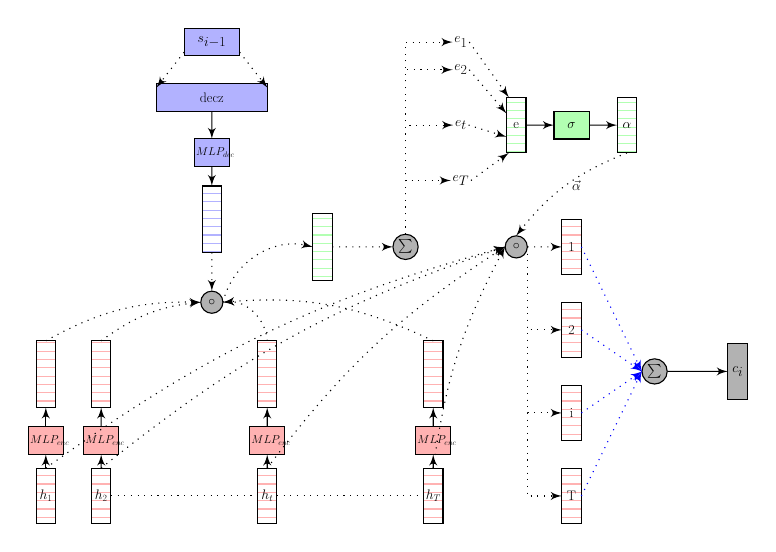
\begin{tikzpicture}[scale=0.2, every node/.style={transform shape}]
	\node [enc_h] (h1) {$h_{1}$};
	\node [enc_h,right of = h1] (h2) {$h_{2}$};
	\node [enc_h,right of = h2, node distance = 30em] (hi) {$h_{t}$};
	\node [enc_h,right of = hi, node distance = 30em] (hTx) {$h_{T}$};
	\draw [dotted] (h2.east) to (hi.west);
	\draw [dotted] (hi.east) to (hTx.west);
	
	
	\node [mlp_enc, above of = h1, node distance = 10em] (mlp1) {$MLP_{enc}$};
	\path [line] (h1.north) to (mlp1.south);
	\node [enc_h, above of = mlp1, minimum height = 12em, node distance = 12em] (he1) {};
	\path [line] (mlp1.north) to (he1.south);
	
	
	\node [mlp_enc, above of = h2, node distance = 10em] (mlp2) {$MLP_{enc}$};
	\path [line] (h2.north) to (mlp2.south);
	\node [enc_h, above of = mlp2, minimum height = 12em, node distance = 12em] (he2) {};
	\path [line] (mlp2.north) to (he2.south);
	
	
	\node [mlp_enc, above of = hi, node distance = 10em] (mlpi) {$MLP_{enc}$};
	\path [line] (hi.north) to (mlpi.south);
	\node [enc_h, above of = mlpi, minimum height = 12em, node distance = 12em] (hei) {};
	\path [line] (mlpi.north) to (hei.south);
	
	
	\node [mlp_enc, above of = hTx, node distance = 10em] (mlpTx) {$MLP_{enc}$};
	\path [line] (hTx.north) to (mlpTx.south);
	\node [enc_h, above of = mlpTx, minimum height = 12em, node distance = 12em] (heTx) {};
	\path [line] (mlpTx.north) to (heTx.south);
	
	\node [mlp_dec, above of = hei, node distance = 60em, minimum width = 10em, xshift = -10em, font=\fontsize{40}{10}\selectfont] (sim1) {$s_{i-1}$};
	\node [mlp_dec, below of=sim1, minimum width = 20em, font=\fontsize{40}{10}\selectfont] (dec_z) {decz};
	\path [line, dotted] (sim1.200) to (dec_z.170);
	\path [line, dotted] (sim1.-20) to (dec_z.10);
	\node [mlp_dec, below of=dec_z, node distance = 10em] (mlp_dec) {$MLP_{dec}$};
	\path [line] (dec_z) to (mlp_dec);
	\node [dec_z, below of = mlp_dec, minimum height = 12em, node distance = 12em] (decz_enc) {};
	\path [line] (mlp_dec) to (decz_enc);
	
	
	\node [round, below of = decz_enc, node distance = 15em] (prod) {$\circ$}; 
	\path [line, dotted] (decz_enc.south) to (prod.north);
	
	\path [line, dotted] (he1.north) to [bend left=15] (prod.west);
	\node [atts, right of = prod, minimum height = 12em, node distance = 20em, yshift=10em] (h_z) {};
	\path [line, dotted] (prod.east) to [bend left=45] (h_z.west);
	
	
	\node [round, right of = h_z, node distance = 15em] (sum) {$\sum$};
	\path [line, dotted] (h_z.east) to (sum.west);
	
	
	
	\node [right of=sim1, node distance = 15em, xshift=30em, font=\fontsize{40}{10}\selectfont] (e1) {$e_{1}$};
	
	\path [line, dotted] (sum.north) |- (e1.west);
	
	\node [below of=e1, node distance = 5em, font=\fontsize{40}{10}\selectfont] (e2) {$e_{2}$};
	
	\path [line, dotted] (he2.north) to [bend left=15] (prod.west);
	\path [line, dotted] (sum.north) |- (e2.west);
	
	
	
	\node [below of=e2, node distance = 10em, font=\fontsize{40}{10}\selectfont] (ei) {$e_{t}$};
	
	\path [line, dotted] (hei.north) to [bend right=45] (prod.east);
	\path [line, dotted] (sum.north) |- (ei.west);
	
	
	
	\node [below of=ei, node distance = 10em, font=\fontsize{40}{10}\selectfont] (eTx) {$e_{T}$};
	
	\path [line, dotted] (heTx.north) to [bend right=15] (prod.east);
	\path [line, dotted] (sum.north) |- (eTx.west);
	
	
	\node [atts, right of=ei, font=\fontsize{40}{10}\selectfont] (e) {e};
	
	
	\path [line, dotted] (e1.east) to (e.105);
	\path [line, dotted] (e2.east) to (e.130);
	\path [line, dotted] (ei.east) to (e.-130);
	\path [line, dotted] (eTx.east) to (e.-105);
	
	
	\node [mlp_att, right of=e, font=\fontsize{40}{10}\selectfont] (sm) {$\sigma$};
	\path [line] (e.east) to (sm.west);
	
	
	\node [atts, right of=sm, font=\fontsize{40}{10}\selectfont] (alphas) {$\alpha$};
	\path [line] (sm.east) to (alphas.west);
	
	
	\node [round, right of=sum, node distance=20em] (alpha_h) {$\circ$};
	\path [line, dotted, color=black] (h1.north) to [bend left=10] (alpha_h.west);
	\path [line, dotted, color=black] (alphas.south) to [bend right=15] node [xshift=2em] {\fontsize{40}{10}\selectfont $\vec{\alpha}$} (alpha_h.north);
	
	
	\node [enc_h, right of=alpha_h] (ahe1) {1};
	\path [line, dotted, color=black] (alpha_h.east) to (ahe1.west);
	
	\path [line, dotted, color=black] (h2.north) to [bend left=10] (alpha_h.west);
	\node [enc_h, below of=ahe1, node distance = 15em] (ahe2) {2};
	\path [line, dotted, color=black] (alpha_h.east) |- (ahe2.west);
	
	
	\path [line, dotted, color=black] (hi.north) to [bend left=10] (alpha_h.west);
	\node [enc_h, below of=ahe2, node distance = 15em] (ahei) {i};
	\path [line, dotted, color=black] (alpha_h.east) |- (ahei.west);
	
	\path [line, dotted, color=black] (hTx.north) to [bend left=10] (alpha_h.west);
	\node [enc_h, below of=ahei, node distance = 15em] (aheTx) {T};
	\path [line, dotted, color=black] (alpha_h.east) |- (aheTx.west);
	
	\node [round, right of=ahe2, yshift=-7.5em, node distance = 15em] (sum_op) {$\sum$};
	\path [line, dotted, color=blue] (ahe1.east) to (sum_op.west);
	\path [line, dotted, color=blue] (ahe2.east) to (sum_op.west);
	\path [line, dotted, color=blue] (ahei.east) to (sum_op.west);
	\path [line, dotted, color=blue] (aheTx.east) to (sum_op.west);
	
	
	\node [enc_h, right of=sum_op, fill=black!30, node distance=15em, font=\fontsize{40}{10}\selectfont] (ci) {$c_i$};
	\path [line] (sum_op.east) to (ci.west);
	\end{tikzpicture}
\end{center}
\end{frame}

\begin{frame}[fragile]{Types of attention}
\begin{itemize}
	\item Classified based on the \textbf{relevance/compatibility} function
	\item Content-based (Depends only on the contents of encoder/decoder states)
	\item Location-aware (Depends on previous attentions)
	\item Hybrid attention
	\item Multi-head attention
	\item Transformer architectures
\end{itemize}
\end{frame}

\section{Joint CTC/Attention architectures [Watanabe et al., 2017]}
\begin{frame}[fragile]{Joint CTC/Attention}
\begin{itemize}
	\item $\mathcal{L}_{MOL} = \lambda \log\left(p_{ctc}(y|X)\right) + (1 - \lambda) \log\left(p_{att}(y|X)\right)$
	\begin{figure}
		\includegraphics[height=0.8\textheight]{./images/mtl4.png}
	\end{figure}
\end{itemize}
\end{frame}


\begin{frame}[fragile]{Joint CTC/Attention - Monotonic alignments}
\begin{figure}
	\includegraphics[width=\linewidth]{./images/mtl2.png}
\end{figure}

\begin{figure}
	\includegraphics[width=\linewidth]{./images/mtl3.png}
\end{figure}	

\end{frame}

\begin{frame}[fragile]{Joint CTC/Attention - Decoding}
\begin{figure}
	\includegraphics[height=0.8\textheight]{./images/mtl1.png}
\end{figure}	
 
\end{frame}

\section{Our Work - Proposed multi-target architecture [Under review at ASRU 2019]}
\begin{frame}[fragile]{Architecture}
	\begin{center}
		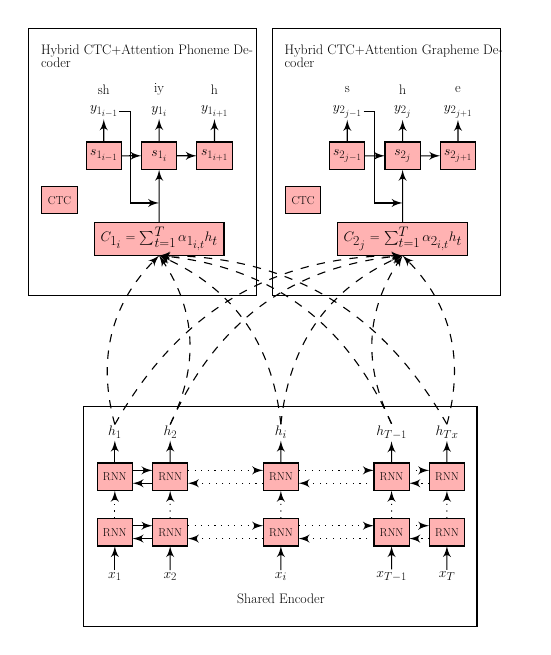
\begin{tikzpicture}[scale=0.2, every node/.style={transform shape}]
		
		
		\pgfmathdeclarefunction{gauss}{2}{%
		\pgfmathparse{1/(#2*sqrt(2*pi))*exp(-((x-#1)^2)/(2*#2^2))}%
		}
		
		
		\node[mlp_enc](LSTM_1_1){RNN};
		\node[mlp_enc, right of=LSTM_1_1](LSTM_1_2) {RNN};
		\path [line] (LSTM_1_1.20) to (LSTM_1_1.20-|LSTM_1_2.west);
		\path [line] (LSTM_1_2.200) to (LSTM_1_2.-20-|LSTM_1_1.east);     
		
		\node[mlp_enc, right of=LSTM_1_2, node distance = 20em](LSTM_1_i) {RNN};
		\path [line, dotted] (LSTM_1_2.20) to (LSTM_1_2.20-|LSTM_1_i.west);
		\path [line, dotted] (LSTM_1_i.200) to (LSTM_1_i.200-|LSTM_1_2.east);
		
		\node[mlp_enc, right of=LSTM_1_i, node distance = 20em](LSTM_1_mTx) {RNN};
		\path [line, dotted] (LSTM_1_i.20) to (LSTM_1_i.20-|LSTM_1_mTx.west);
		\path [line, dotted] (LSTM_1_mTx.200) to (LSTM_1_mTx.200-|LSTM_1_i.east);
		
		\node[mlp_enc, right of=LSTM_1_mTx](LSTM_1_Tx) {RNN};
		\path [line, dotted] (LSTM_1_mTx.20) to (LSTM_1_mTx.20-|LSTM_1_Tx.west);
		\path [line, dotted] (LSTM_1_Tx.200) to (LSTM_1_Tx.200-|LSTM_1_mTx.east);
		
		
		\node [below of=LSTM_1_1, node distance = 8em] (x1) {\Huge $x_{1}$};
		\node [below of=LSTM_1_2, node distance = 8em] (x2) {\Huge $x_{2}$};
		\node [below of=LSTM_1_i, node distance = 8em] (xi) {\Huge $x_{i}$};
		\node [below of=LSTM_1_mTx, node distance = 8em] (xTm1) {\Huge $x_{T-1}$};
		\node [below of=LSTM_1_Tx, node distance = 8em] (xTx) {\Huge $x_{T}$};
		
		
		\path [line] (x1) to (LSTM_1_1);
		\path [line] (x2) to (LSTM_1_2);
		\path [line] (xi) to (LSTM_1_i);
		\path [line] (xTm1) to (LSTM_1_mTx);
		\path [line] (xTx) to (LSTM_1_Tx);
		
		\node[mlp_enc, above of = LSTM_1_1, node distance = 10em](LSTM_N_1){RNN};
		\node[mlp_enc, right of=LSTM_N_1](LSTM_N_2) {RNN};
		\path [line] (LSTM_N_1.20) to (LSTM_N_1.20-|LSTM_N_2.west);
		\path [line] (LSTM_N_2.200) to (LSTM_N_2.-20-|LSTM_N_1.east);     
		
		\node[mlp_enc, right of=LSTM_N_2, node distance = 20em](LSTM_N_i) {RNN};
		\path [line, dotted] (LSTM_N_2.20) to (LSTM_N_2.20-|LSTM_N_i.west);
		\path [line, dotted] (LSTM_N_i.200) to (LSTM_N_i.200-|LSTM_N_2.east);
		
		\node[mlp_enc, right of=LSTM_N_i, node distance = 20em](LSTM_N_mTx) {RNN};
		\path [line, dotted] (LSTM_N_i.20) to (LSTM_N_i.20-|LSTM_N_mTx.west);
		\path [line, dotted] (LSTM_N_mTx.200) to (LSTM_N_mTx.200-|LSTM_N_i.east);
		
		\node[mlp_enc, right of=LSTM_N_mTx](LSTM_N_Tx) {RNN};
		\path [line, dotted] (LSTM_N_mTx.20) to (LSTM_N_mTx.20-|LSTM_N_Tx.west);
		\path [line, dotted] (LSTM_N_Tx.200) to (LSTM_N_Tx.200-|LSTM_N_mTx.east);
		
		\path [line, dotted] (LSTM_1_1) to (LSTM_N_1);
		\path [line, dotted] (LSTM_1_2) to (LSTM_N_2);
		\path [line, dotted] (LSTM_1_i) to (LSTM_N_i);
		\path [line, dotted] (LSTM_1_mTx) to (LSTM_N_mTx);
		\path [line, dotted] (LSTM_1_Tx) to (LSTM_N_Tx);
		
		\node [above of = LSTM_N_1, node distance = 8em] (h1) {\Huge $h_{1}$};
		\node [above of = LSTM_N_2, node distance = 8em] (h2) {\Huge $h_{2}$};
		\node [above of = LSTM_N_i, node distance = 8em] (hi) {\Huge $h_{i}$};
		\node [above of = LSTM_N_mTx, node distance = 8em] (hTm1) {\Huge $h_{T-1}$};
		\node [above of = LSTM_N_Tx, node distance = 8em] (hTx) {\Huge $h_{Tx}$};
		
		\path [line] (LSTM_N_1) to (h1);
		\path [line] (LSTM_N_2) to (h2);
		\path [line] (LSTM_N_i) to (hi);
		\path [line] (LSTM_N_mTx) to (hTm1);
		\path [line] (LSTM_N_Tx) to (hTx);
		
		\node[mlp_enc, above of = h1, node distance = 50em, xshift=8em](pd1)  {\Huge $s_{1_{i}}$};
		\node[mlp_enc, left of = pd1](pd2)  {\Huge $s_{1_{i-1}}$};
		\node[mlp_enc, right of = pd1](pd3)  {\Huge $s_{1_{i+1}}$};
		
		\path [line] (pd2) to (pd1);
		\path [line] (pd1) to (pd3);
		
		\node[mlp_enc, above of = hTx, node distance = 50em, xshift=-8em](pd5)  {\Huge $s_{2_{j}}$};
		\node[mlp_enc, right of = pd5](pd4)  {\Huge $s_{2_{j+1}}$};
		\node[mlp_enc, left of = pd5](pd6)  {\Huge $s_{2_{j-1}}$};
		
		\path [line] (pd6) to (pd5);
		\path [line] (pd5) to (pd4);
		
		\node[mlp_enc,text width=8cm, above of = h1, node distance = 35em, font=\fontsize{40}{20}\selectfont, minimum height=6em, xshift=8em](C1) {$C_{1_{i}} = \sum_{t=1}^{T} \alpha_{1_{i,t}} h_{t}$};
		\node[mlp_enc,text width=8cm,above of = hTx, node distance = 35em, font=\fontsize{40}{20}\selectfont, minimum height=6em, xshift=-8em](C2) {$C_{2_{j}} = \sum_{t=1}^{T} \alpha_{2_{i,t}} h_{t}$};
		
		\path [line] (C1) to (pd1);
		\path [line] (C2) to (pd5);
		
		%\begin{axis}[
		%anchor=origin,
		%x=0.5cm,
		%at={(8cm,8cm)},
		%style={samples=1000,smooth},
		%hide axis
		%]
		%\addplot[mark=none] {gauss(0,1)};
		%\end{axis}
		%
		%\begin{axis}[
		%anchor=origin,
		%x=1cm,
		%at={(9cm,8cm)},
		%style={samples=1000,smooth},
		%hide axis
		%]
		%\addplot[mark=none, dashed] {gauss(0,1)};
		%\end{axis}
		%
		%\path [line] (7,9) -- (C1);
		%\path [line] (11,9) -- (C2);
		
		\path [line, dashed] (h1.north) to[bend left=30] (C1.south);
		\path [line, dashed] (h2.north) to[bend right=30] (C1.south);
		\path [line, dashed] (hi.north) to[bend right=30] (C1.south);
		\path [line, dashed] (hTm1.north) to[bend right=30] (C1.south);
		\path [line, dashed] (hTx.north) to[bend right=30] (C1.south);
		
		\path [line, dashed] (h1.north) to[bend left=30] (C2.south);
		\path [line, dashed] (h2.north) to[bend left=30] (C2.south);
		\path [line, dashed] (hi.north) to[bend left=30] (C2.south);
		\path [line, dashed] (hTm1.north) to[bend left=30] (C2.south);
		\path [line, dashed] (hTx.north) to[bend right=30] (C2.south);
		
		\node [above of = pd2, node distance=8em] (ym1) {\Huge $y_{1_{i-1}}$};
		\node [above of = pd1, node distance=8em] (y1) {\Huge $y_{1_{i}}$};
		\node [above of = pd3, node distance=8em] (yp1) {\Huge $y_{1_{i+1}}$};
		
		\node [above of = ym1, node distance=4em] (o1) {\Huge sh};
		\node [above of = y1, node distance=4em] (o2) {\Huge iy};
		\node [above of = yp1, node distance=4em] (o3) {\Huge h};
		
		\path [line] (pd2) to (ym1);
		\path [line] (pd1) to (y1);
		\path [line] (pd3) to (yp1);
		
		
		\node [above of = pd4, node distance=8em] (ym2) {\Huge $y_{2_{j+1}}$};
		\node [above of = pd5, node distance=8em] (y2) {\Huge $y_{2_{j}}$};
		\node [above of = pd6, node distance=8em] (yp2) {\Huge $y_{2_{j-1}}$};
		
		\path [line] (ym1.east) -- +(2em,0) |- ($(pd1.south) - (0,6em)$);
		\path [line] (yp2.east) -- +(2em,0) |- ($(pd5.south) - (0,6em)$);
		
		\node [above of = ym2, node distance=4em] (o1) {\Huge e};
		\node [above of = y2, node distance=4em] (o2) {\Huge h};
		\node [above of = yp2, node distance=4em] (o3) {\Huge s};
		
		
		\path [line] (pd4) to (ym2);
		\path [line] (pd5) to (y2);
		\path [line] (pd6) to (yp2);
		
		
		\draw (-2,-6) rectangle (23,8);
		
		\node[below of=xi, font=\fontsize{40}{10}\selectfont, node distance=4em] {Shared Encoder};
		\node[above of=y1, font=\fontsize{40}{10}\selectfont, node distance=10em, text width=15cm] {Hybrid CTC+Attention Phoneme Decoder};
		\node[above of=y2, font=\fontsize{40}{10}\selectfont, node distance=10em, text width=15cm] {Hybrid CTC+Attention Grapheme Decoder};
		
		\draw (-5.5,15) rectangle (9,32);
		\draw (10,15) rectangle (24.5,32);
		
		
		\node[mlp_enc, below of=pd2, xshift=-8em, node distance=8em](ctc1) {CTC};
		\node[mlp_enc, below of=pd6, xshift=-8em, node distance=8em](ctc1) {CTC};
		
		\end{tikzpicture}
	\end{center}
\end{frame}


\section{Results}
\subsection{Architectural studies on TIMIT}
\begin{frame}[fragile]{Joint attention on phoneme-grapheme}
	\begin{center}
		\begin{figure}[!ht]
			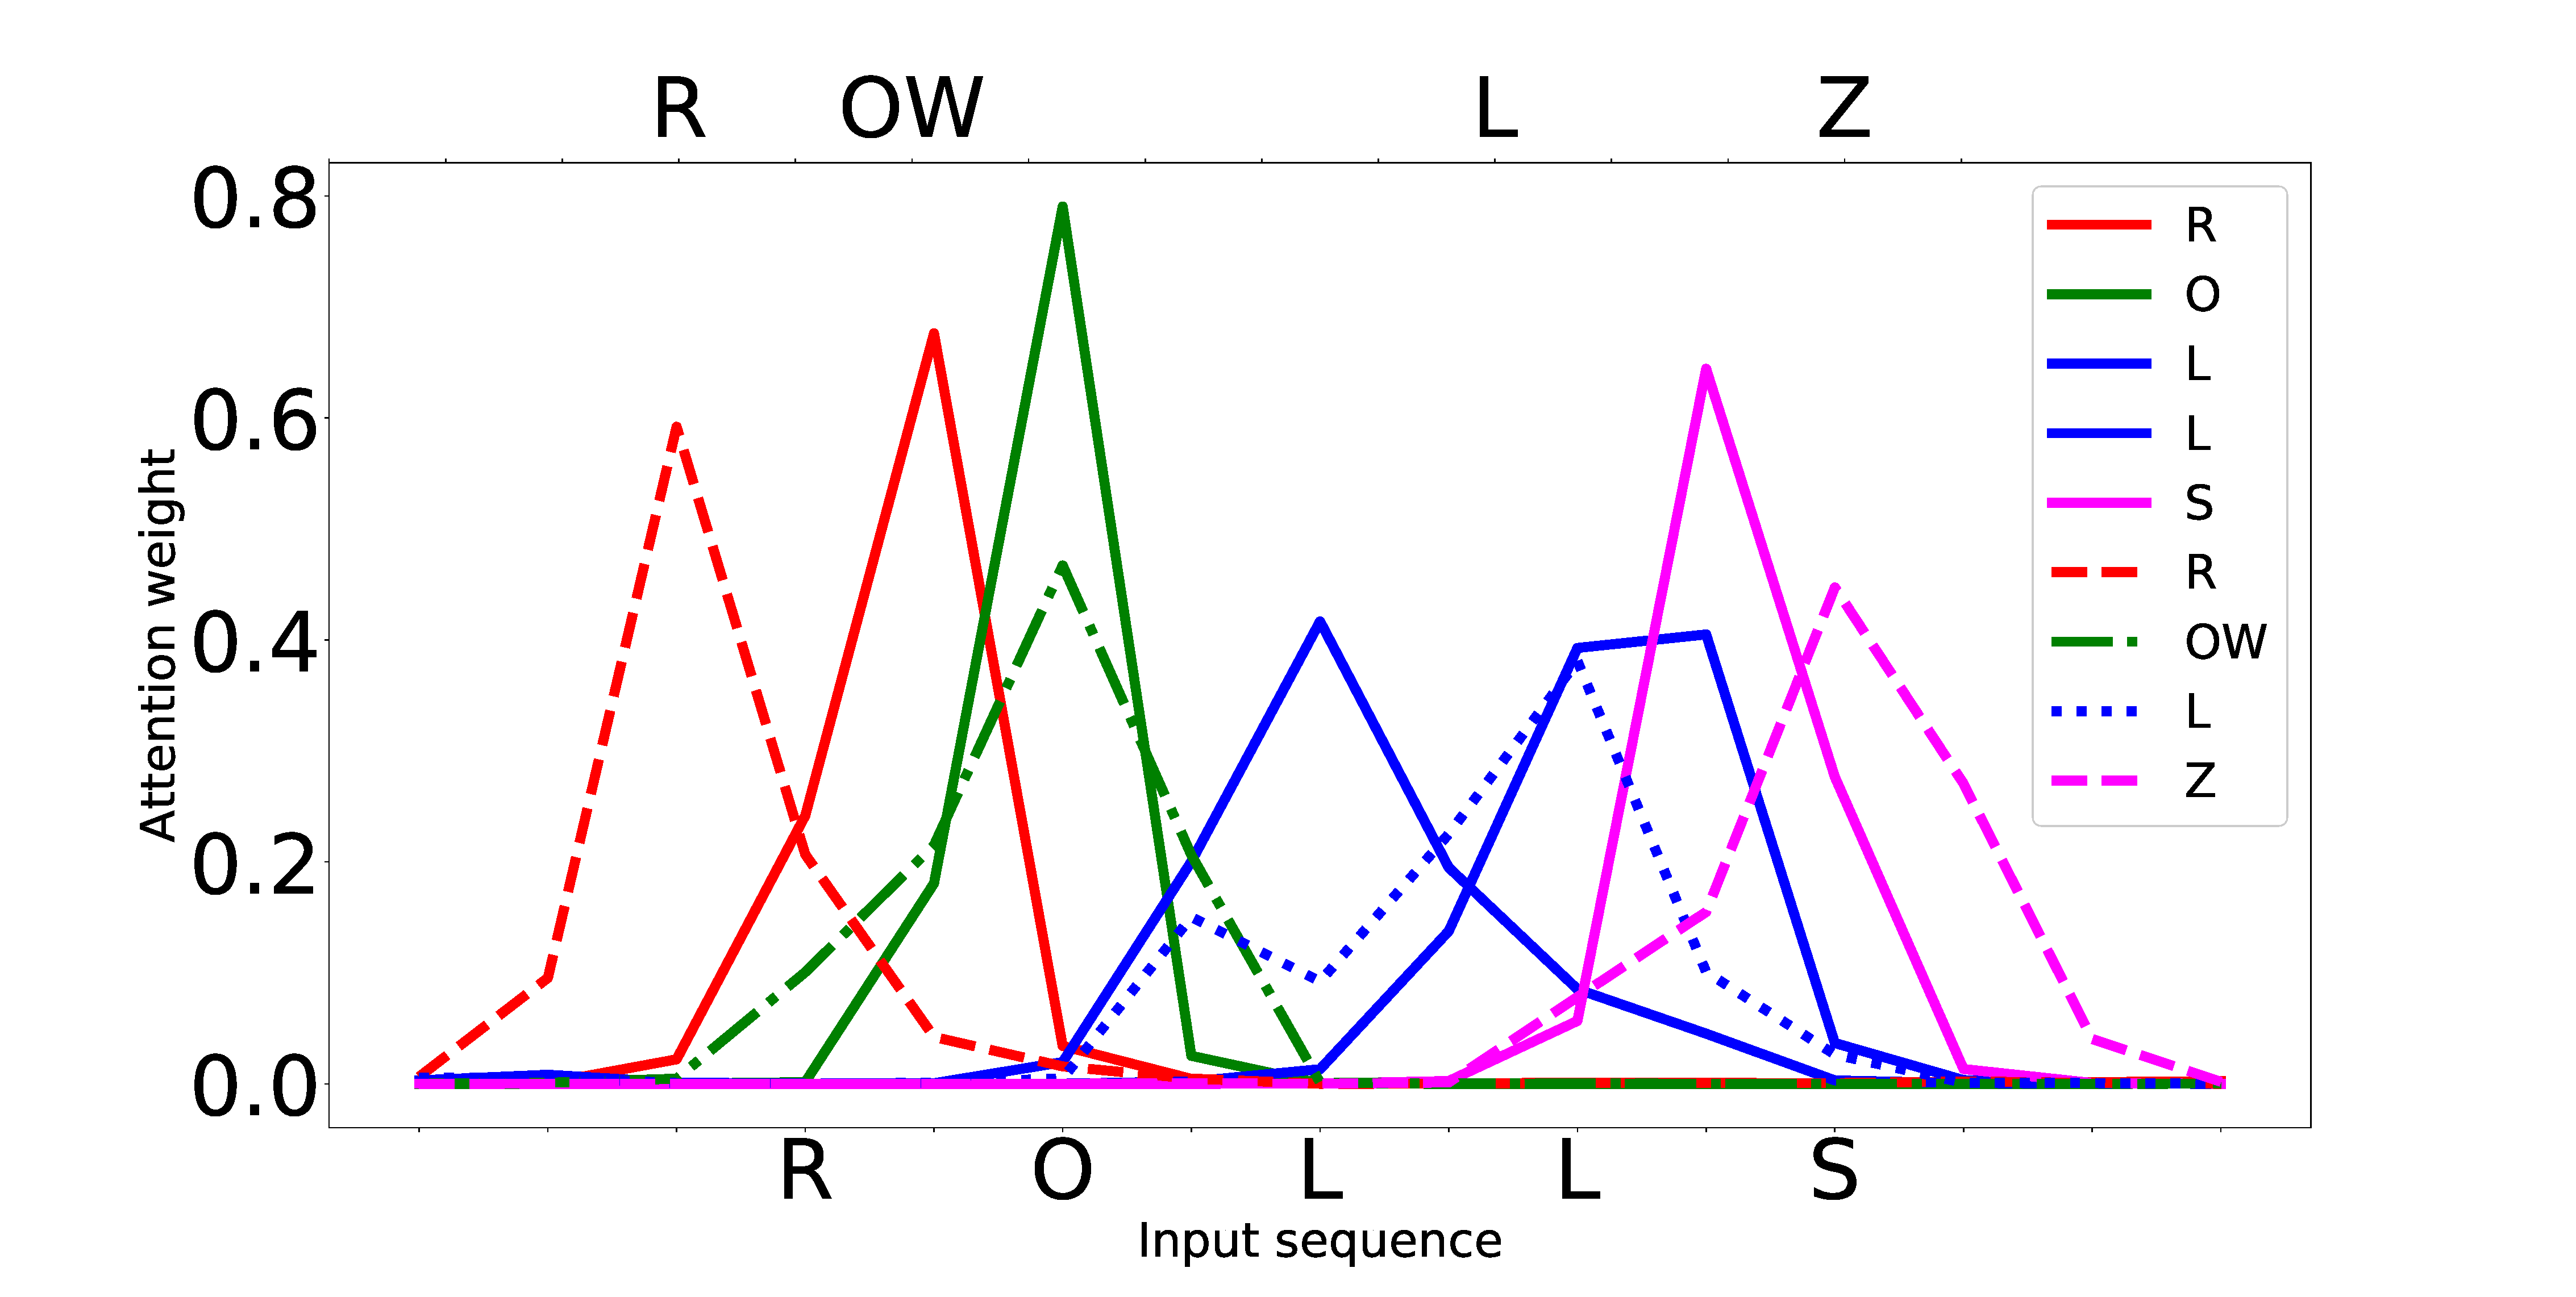
\includegraphics[width=\textheight]{./results/att_ind.eps}
			\captionof{figure}{Attention weights for predicting phonemes ($\textit{r ow l z}$) and graphemes (r o l l s) of the word "rolls"}
			\label{fig:attind}
		\end{figure}
	\end{center}
\end{frame}

\begin{frame}[fragile]{Attention profile on phoneme-grapheme}
	\begin{center}
	\begin{figure}[!ht]
		
		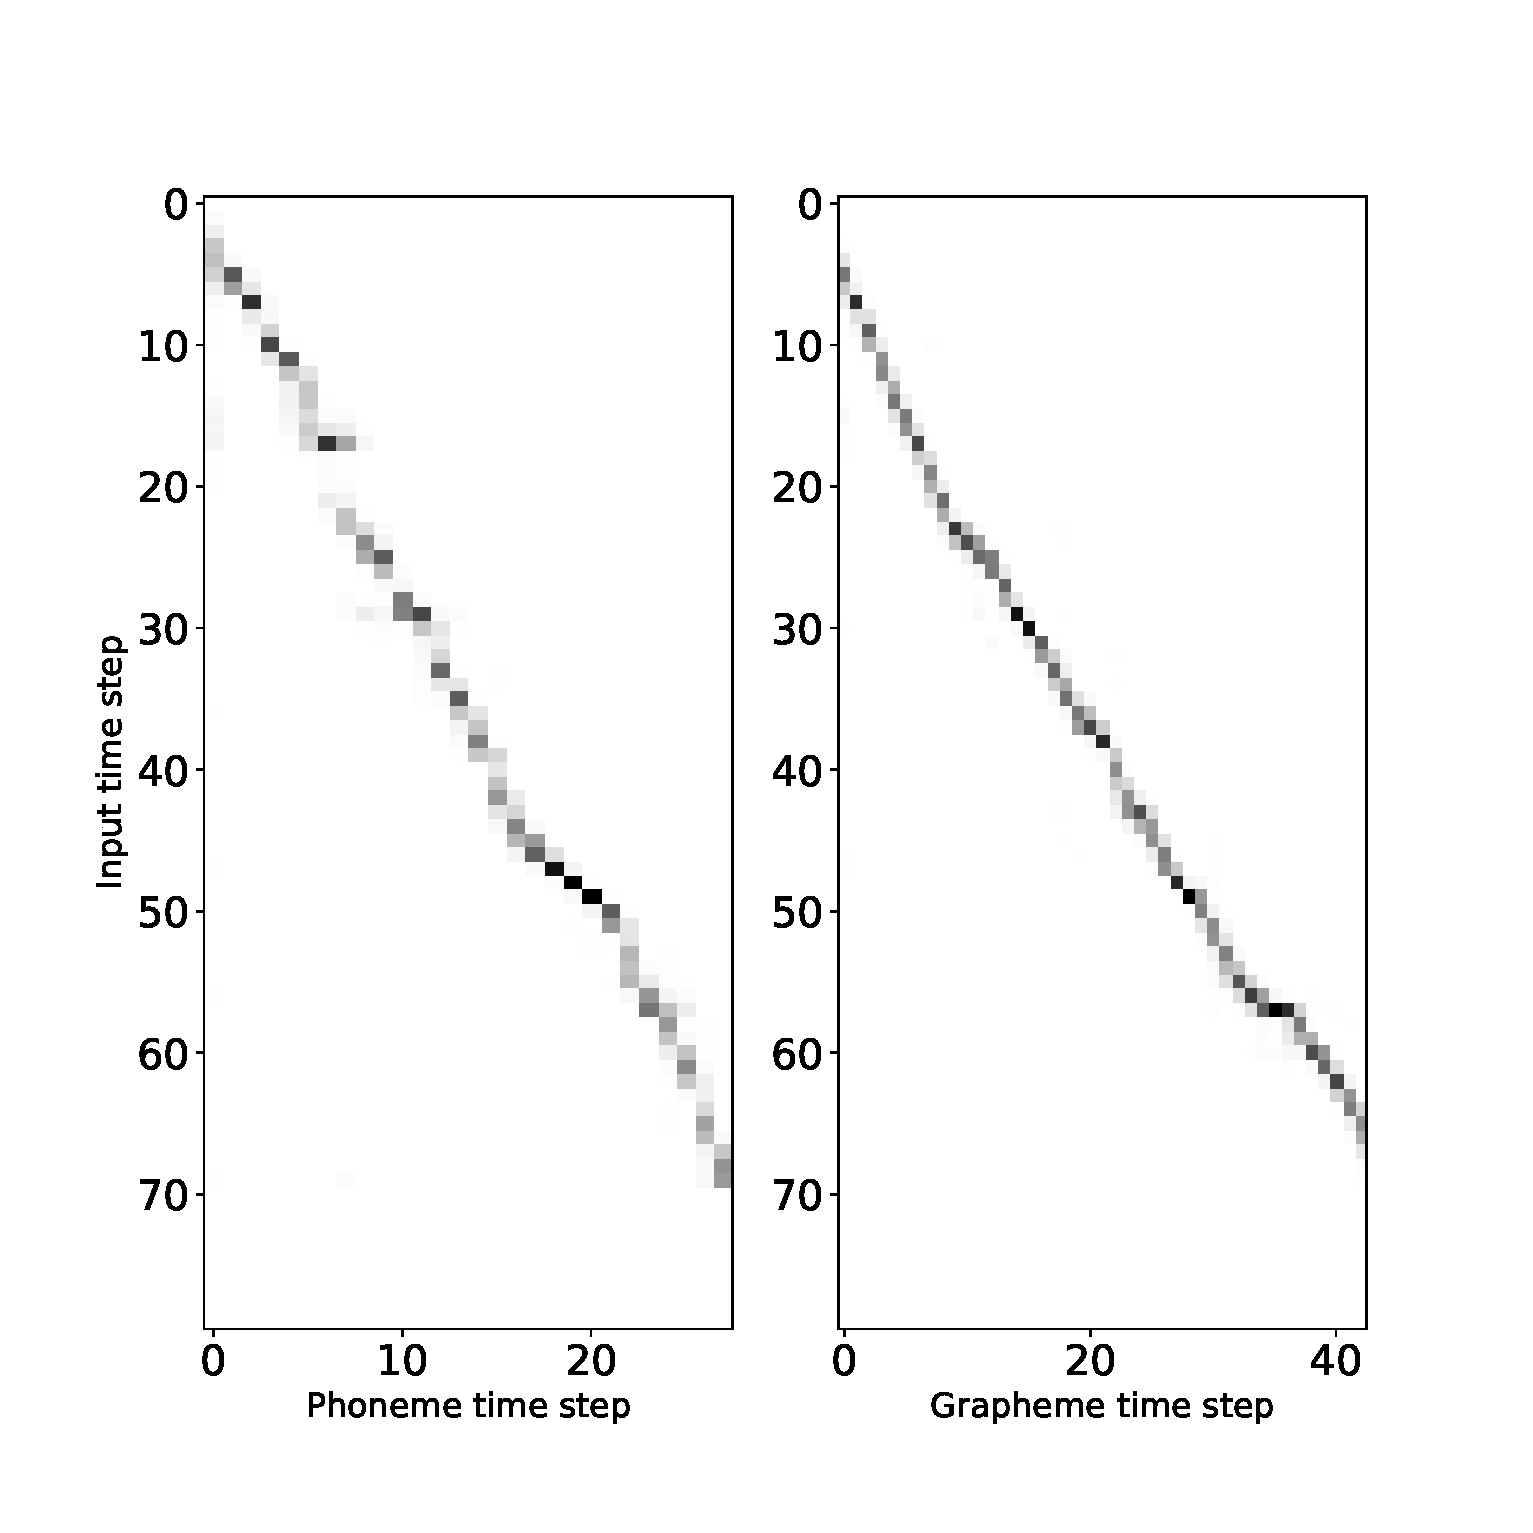
\includegraphics[height=0.7\textheight]{./results/attention.eps}
		\captionof{figure}{Attention profile for predicting phoneme and grapheme sequences for the example TIMIT utterance \textbf{FADG0\_SI1909}}
		\label{fig:attall}
	\end{figure}
	\end{center}
\end{frame}

\begin{frame}[fragile]{Results on Librispeech train\_clean\_100 and test\_clean}
\begin{center}
	\begin{center}
		\begin{tabular}{|c | c | c|}
			\hline
			Target & PER & CER\\
			\hline\hline
			phoneme & 7 & - \\
			\hline
			grapheme & - & 7.7 \\
			\hline
			phoneme @ 5L, grapheme @ 5L & 7.4 & 8.1 \\
			phoneme @ 3L, grapheme @ 5L & 7.2 & 7.8 \\
			phoneme @ 1L, grapheme @ 5L & \textbf{6.8} & \textbf{7.1} \\
			\hline
		\end{tabular}
	\end{center}
\end{center}
\end{frame}

\section{Future Work}

\subsection{Multi-Head decoder}
\begin{frame}[fragile]{Multi-Head decoder with ASWU targets}
\begin{itemize}
	\item Introduce automatically derived acoustic sub-word units
	\item Performance with multi-target decoder
	\item Hierarchical target learning. ASWU->phonemes->characters->(word-pieces?)
\end{itemize}
\end{frame}

\subsection{Attention as alignment}
\begin{frame}[fragile]{Attention as alignment - Attention-assisted Forced Alignment}
\begin{itemize}
	\item Align features based on attention distribution
	\item Attention is too sensitive for transcript. (Need some slack?)
	\item Confidence measure for Forced Alignment
	\item Keyword spotting with this framework. (Sliding window method)
	\item Transcript : "<space> w iy <space> d ih <space> n aa dx ah <space> k s eh <space> dh ah <space> d ay <space> n aa s ih s ae w ah n s <space> <space> b ah <space> g r ae sh ah l iy <space> w iy aa <space> \textbf{k ah m ih ng} <space> t uw <space>"
\end{itemize}
\begin{figure}
	\includegraphics[height=0.4\textheight]{./kws.png}
\end{figure}

\end{frame}

\subsection{ORACLE}
\begin{frame}[fragile]{ORACLE Attention - Ekam Sat Vipra Bahudha Vadanti?}

\begin{itemize}
	\item Transcript is always monotonically aligned to speech
	\item There are 13 variants of Attention mechanisms widely used.
	\item Is there a "one true" attention (alignment)?
	\item ORACLE as an initial estimate (from GMM-HMM)
	\item Effects on convergence
	\item Early results using Wasserstein metric
	\begin{figure}
		\includegraphics[height=0.4\textheight]{images/oracle_sh.png}
	\end{figure}
\end{itemize}
\end{frame}

\subsection{Interpretability and Explainability}
\begin{frame}[fragile]{Interpretability and Explainability}

\begin{itemize}
	\item Track attention to formant movement?
\end{itemize}
\includegraphics[width=\linewidth, height=0.7\textheight]{formant.jpg}
\end{frame}

\subsection{Analysis}

\subsection{Analysis}
\begin{frame}[fragile]{Analysis}

\begin{itemize}
	\item When the model is making a mistake, it it looking at the wrong location in the signal?
	\item Could we decouple the location part of the network from the content part? (Helps in transfer learning)
	\item The Context vector $C$ - how is it distributed after every epoch? Could we see them getting separated?
	\item Location-aware attention always starts from left (strict). Content-based attention can span over entire signal. Use this for faster kws models.
\end{itemize}
\end{frame}

\begin{frame}[fragile]{Suggestions}
Suggestions please.
\end{frame}

\end{document}